\documentclass[conference]{IEEEtran}

%--------------------------------------------------
% Packages
%--------------------------------------------------
\usepackage[utf8]{inputenc}
\usepackage[T1]{fontenc}
\usepackage{times}
\usepackage{amsmath}
\usepackage{array}
\usepackage{booktabs}
\usepackage{enumitem}
\usepackage{graphicx}
\usepackage{url}
\usepackage{float}
\usepackage{tikz}
\usetikzlibrary{arrows.meta,positioning,shapes.geometric}

\begin{document}

%--------------------------------------------------
% Title & Authors (IEEE style)
%--------------------------------------------------
\title{A Smart Food Ordering and Waste Reduction System for Train Services:\\
A Comparative Mixed-Method Analysis}

\author{
\IEEEauthorblockN{Md Tanver Jakaria, Ishaq Sharif, Tamim Hossain, Namira Kabir Vumika}
\IEEEauthorblockA{Department of Computer Science and Engineering\\
Military Institute of Science and Technology\\
Dhaka, Bangladesh\\
%Email: \{email1, email2, email3, email4\}@example.com}
}}

\maketitle

\begin{abstract}
Railway food services face persistent operational constraints, including uncertain passenger demand, limited on-board storage, restricted preparation capacity, and strict schedule-driven delivery windows. These constraints frequently produce overproduction, stock-outs, quality inconsistency, and avoidable food waste, while also reducing passenger satisfaction. Although recent studies report promising results from mobile ordering, machine-learning-based demand forecasting, IoT quality monitoring, and digital traceability, most evidence comes from campuses, institutional kitchens, agricultural chains, and commercial delivery platforms rather than railway settings. This study applies a comparative mixed-method design to synthesize findings from ten selected studies and a passenger survey, and then evaluates them across five dimensions: forecasting accuracy, waste reduction, transparency, consumer satisfaction, and environmental impact. The analysis shows strong potential for combining pre-ordering, demand forecasting, dynamic pricing, QR-based traceability, and real-time quality monitoring in railway catering, but also highlights adoption and implementation barriers that require organizational support. Survey evidence indicates high concern about waste and strong interest in transparency features, while moderate app-adoption intent suggests the need for better usability, trust-building, and service reliability. The paper contributes an evidence-based analytical framework and practical design guidance for future railway-focused pilots and phased implementation, including alignment between technical features and organizational practices.
\end{abstract}

\begin{IEEEkeywords}
railway catering, food waste reduction, demand forecasting, digital traceability, mixed-method analysis
\end{IEEEkeywords}

%--------------------------------------------------
% 1 Introduction
%--------------------------------------------------
\section{Introduction}

Railway food services operate under constraints such as variable passenger demand, limited on-board storage, constrained preparation facilities, and tight delivery windows defined by train schedules. These conditions lead to frequent overproduction, stock-outs, and inconsistent food quality, which in turn create food waste and passenger dissatisfaction. Traditional processes also provide limited visibility into inventory movement, cold-chain conditions, and supplier performance along the route.

In parallel, a growing body of research has examined digital food ordering platforms, institutional food service forecasting, IoT-based quality monitoring, blockchain traceability, and circular economy initiatives in stationary and commercial contexts. These studies demonstrate that mobile ordering, IoT monitoring, machine learning (ML) forecasting, and digital traceability can improve demand prediction, product quality, and transparency. However, most of this evidence comes from campuses, institutional kitchens, agricultural supply chains, or online delivery platforms, not from railway environments.

This article therefore examines how existing systems and technologies, studied in other domains, could inform the design and evaluation of a smart food ordering and waste reduction system for train services. The focus is strictly on analysing and comparing current research contributions; no new system is implemented in practice.

%--------------------------------------------------
% 2 Objective
%--------------------------------------------------
\section{Objective}

The study objective is to develop evidence-based guidance for designing a smart food ordering and waste reduction approach tailored to railway services.

Specific objectives are as follows:

\begin{itemize}[leftmargin=*]
\item To identify key operational problems in current railway food services, including demand uncertainty, waste generation, and service inconsistency.
\item To compare relevant literature on digital food ordering, demand forecasting, traceability, IoT monitoring, and sustainability-oriented food service models.
\item To evaluate findings across five dimensions: forecasting accuracy, waste reduction, transparency, passenger satisfaction, and environmental impact.
\item To interpret passenger survey evidence in relation to these dimensions and derive practical implications for railway deployment.
\item To propose a railway-focused analytical framework that can support future pilot design and implementation planning.
\end{itemize}

%--------------------------------------------------
% 3 Problem Statement
%--------------------------------------------------
\section{Problem Statement}

The railway food service sector faces several well-recognised challenges:

\begin{itemize}[leftmargin=*]
\item \textit{Unpredictable demand}: passenger numbers and ordering behaviour vary by route, time, and station, making accurate production planning difficult and leading to overproduction or shortages.
\item \textit{Food waste and cost}: overproduction, limited storage, and time-bound delivery windows cause surplus food that cannot be reused safely, increasing waste and operating cost.
\item \textit{Limited transparency}: existing railway catering processes provide little end-to-end visibility on where, when, and under what conditions food items move from suppliers to trains and passengers.
\item \textit{Inconsistent passenger experience}: passengers frequently report issues with availability, freshness, and reliability of on-board food services, affecting satisfaction and trust.
\end{itemize}

At the same time, the current research landscape is fragmented. Many studies address individual aspects—such as digital traceability, ML-based demand forecasting, consumer behaviour in online food delivery, IoT-based cold chain monitoring, smart kitchen waste tracking, and circular economy models—but rarely consider railway-specific constraints or integrated evaluations.

The problem addressed in this paper is therefore not to build a new system, but to analyse and synthesise existing research on smart food ordering, waste reduction, and digital supply chain technologies. The goal is to derive evidence-based insights and comparative benchmarks that can inform future design and evaluation of railway-focused solutions.

%--------------------------------------------------
% 4 Literature Review
%--------------------------------------------------
\section{Literature Review}

The literature synthesis covers ten complementary studies on smart food systems, including digital traceability, demand forecasting, consumer behaviour, IoT monitoring, institutional waste reduction, smart kitchen tools, circular economy models, blockchain-enabled supply chains, cost--waste integration, and environmental assessment methods~\cite{tarhan2025,mattila2025,varsini2025,wjarr2025cold,ijam2025,benchmark2023,ce4re2025,wjarr2024blockchain,pathway10,envmgmt2025}. Together, these works provide strong multi-domain evidence but are mostly outside railway contexts.

First, technology-driven studies show that combining QR/RFID, IoT sensing, and digital ledgers can improve traceability, quality visibility, and response speed across food supply chains~\cite{tarhan2025,wjarr2025cold,wjarr2024blockchain}. Forecasting-focused work further demonstrates that machine-learning models, especially when integrated with operational data, can significantly reduce overproduction and associated emissions~\cite{mattila2025}. These findings are directly relevant to railway catering, where uncertainty in demand and strict service windows are core constraints.

Second, organization- and user-oriented studies highlight that technical systems alone are insufficient. Evidence from institutional food services and smart kitchen deployments indicates that staff training, participatory practices, workflow redesign, and behavioural nudges are critical for sustained waste reduction~\cite{ijam2025,benchmark2023}. Consumer studies also show that adoption depends on service reliability, perceived quality, transparency, and convenience, not only on app availability~\cite{varsini2025}. This implies that railway implementation must combine digital infrastructure with operational and service-design measures.

Third, sustainability-oriented studies extend the discussion from operational efficiency to long-term impact. Circular economy research emphasizes collaboration, governance, and scalable ecosystem models~\cite{ce4re2025}, while cost--waste and environmental management studies argue for integrated financial and environmental measurement frameworks, including Scope 3 considerations~\cite{pathway10,envmgmt2025}. These insights support a broader railway strategy that links forecasting, waste prevention, and transparent reporting.

Despite these contributions, the key research gap remains: limited integrated evaluation of these technologies and organizational mechanisms under railway-specific constraints. Most prior work examines one subsystem in isolation or in non-rail settings. This study addresses that gap by comparatively synthesizing the ten reviewed articles and interpreting them through a railway-focused analytical framework.

%--------------------------------------------------
% 5 Research Methodology
%--------------------------------------------------
\section{Research Methodology}

\subsection{Mixed-Method Comparative Design}

This study employs a mixed-method research design that combines quantitative and qualitative analysis. No new technical system is deployed; instead, existing implementations and empirical findings are reviewed and compared.

The quantitative component focuses on reported performance metrics from the selected studies, such as waste reduction percentages, forecasting accuracy, service-level indicators, cost impacts, and environmental outcomes. The qualitative component analyses how these systems were designed and implemented, the challenges encountered, and the contextual factors that influenced success or failure. Together, these perspectives support a comparative mixed-method evaluation of current digital food service systems and their relevance to railway food services.

\subsection{Data Collection}

Data collection followed a two-source strategy to avoid ambiguity between evidence types:

\begin{itemize}[leftmargin=*]
\item \textit{Secondary evidence (literature dataset)}: ten selected articles and reports were reviewed to extract comparable technical and contextual findings.
\item \textit{Primary evidence (survey dataset)}: a structured passenger survey (n=27) was conducted to capture current train food experience, adoption intent, and preferences related to waste reduction and transparency.
\end{itemize}

For each literature source, the following information was extracted:

\begin{itemize}[leftmargin=*]
\item \textit{Context and scope}: sector (institutional kitchens, agricultural supply chains, online food delivery, cold chain logistics, circular economy projects), scale, and timeframe.
\item \textit{Technologies and interventions}: use of ML-based demand forecasting, IoT monitoring, blockchain or other traceability tools, smart kitchen systems, and organizational change strategies.
\item \textit{Quantitative results}: reported waste reduction ranges, forecasting error metrics, response times, consumer satisfaction indicators, cost changes, and emission reductions where available.
\item \textit{Qualitative findings}: implementation challenges, organizational barriers, user behaviour, equity considerations, and identified research gaps.
\end{itemize}

For the survey dataset, responses were collected across five sections: demographics and travel habits, current train food experience, mobile ordering preferences, food waste and sustainability, and transparency and trust. This structure enabled direct comparison between literature-based expectations and passenger-reported realities.

All collected data were then organized into a common coding sheet aligned with the five evaluation dimensions, so that descriptive and thematic analysis could be performed consistently across both datasets.

\subsection{Evaluation Dimensions}

To ensure comparability across diverse studies, five evaluation dimensions are used consistently:

\begin{itemize}[leftmargin=*]
\item \textit{Demand forecasting accuracy}: how well the systems predict demand patterns and reduce mismatch between production and actual consumption.
\item \textit{Food waste reduction}: the extent to which interventions reduce food waste volumes and associated financial losses.
\item \textit{Supply chain and process transparency}: improvements in traceability coverage, data availability, and responsiveness to quality or safety issues.
\item \textit{Consumer or passenger satisfaction}: changes in convenience, perceived quality, reliability, and overall experience as reported in the studies.
\item \textit{Environmental impact}: documented effects on emissions or other environmental indicators, often measured through life cycle assessment or related methods.
\end{itemize}

These dimensions align with the research focus on operational performance, user experience, and sustainability, and they are used as lenses to interpret each article’s contributions.

\subsection{Data Analysis Approach}

The analysis proceeds in three main steps:

\begin{itemize}[leftmargin=*]
\item \textit{Descriptive synthesis}: key features, methods, and results from each article are summarised in structured form, highlighting what was done, where, and with what outcomes.
\item \textit{Thematic analysis}: qualitative findings across studies are grouped into recurring themes, such as traceability challenges, forecasting benefits, organizational barriers, equity considerations, and circular economy opportunities.
\item \textit{Comparative interpretation}: the studies are compared along the five evaluation dimensions to identify typical performance ranges, trade-offs between technology-focused and organization-focused approaches, and gaps that are particularly relevant for railway food services.
\end{itemize}

This mixed-method analysis does not calculate new statistics but instead reinterprets existing quantitative and qualitative findings to produce an integrated, railway-oriented perspective on smart food ordering and waste reduction.

%--------------------------------------------------
% 4 Proposed Research Framework
%--------------------------------------------------
\section{Proposed Research Framework}

\subsection{Analytical Perspective for Railway Context}

Because this paper does not implement a new system, the “framework” refers to an analytical lens rather than a concrete technical architecture. It specifies how existing systems and results are interpreted in relation to railway food services.

Two layers are emphasised:

\begin{itemize}[leftmargin=*]
\item \textit{Digital systems layer}: existing solutions for traceability, ML forecasting, IoT monitoring, smart kitchen waste tracking, and circular economy models, as reported in institutional and supply chain studies.
\item \textit{Service context layer}: the specific characteristics of railway services, including variable passenger demand, limited on-board facilities, tight schedules, and multi-station logistics.
\end{itemize}

The framework asks which patterns and limitations observed in non-rail contexts are likely to remain relevant if similar approaches are later adapted for trains.

\subsection{Comparative Evaluation Dimensions}

The same five evaluation dimensions from the methodology are used to structure the framework:

\begin{itemize}[leftmargin=*]
\item Demand forecasting accuracy.
\item Food waste reduction and cost impact.
\item Supply chain and process transparency.
\item Consumer or passenger satisfaction.
\item Environmental impact and sustainability.
\end{itemize}

For each dimension, the reviewed articles provide examples of achievable improvements and common constraints, which are treated as benchmarks and cautionary signals for future railway-focused studies.

\subsection{Phased Insight Generation}

Instead of implementation phases, the framework suggests phases of research insight generation:

\begin{itemize}[leftmargin=*]
\item \textit{Phase 1: Evidence mapping} – summarise existing systems and results, as done in this article.
\item \textit{Phase 2: Contextual translation} – assess which technologies and outcomes appear most applicable to railway operations.
\item \textit{Phase 3: Scenario development} – outline hypothetical railway scenarios using performance ranges drawn from current literature.
\item \textit{Phase 4: Future study design} – propose empirical railway research or pilots informed by the identified gaps and constraints.
\end{itemize}

Figure~\ref{fig:framework-flowchart} visualizes the proposed framework as a sequential process from evidence synthesis to pilot-oriented planning.

\begin{figure}[H]
\centering
\resizebox{0.95\columnwidth}{!}{%
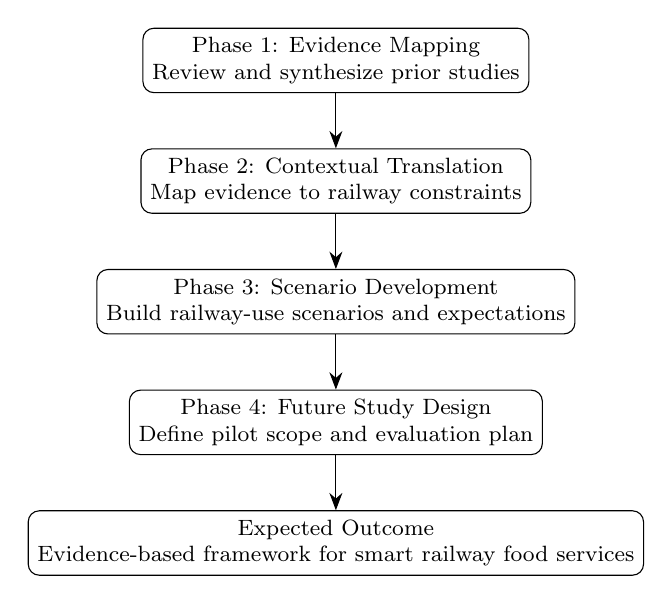
\begin{tikzpicture}[
	node distance=7mm,
	>={Stealth[length=2.2mm]},
	box/.style={draw, rounded corners, align=center, minimum width=4.1cm, minimum height=8mm, font=\footnotesize}
]
\node[box] (p1) {Phase 1: Evidence Mapping\\Review and synthesize prior studies};
\node[box, below=of p1] (p2) {Phase 2: Contextual Translation\\Map evidence to railway constraints};
\node[box, below=of p2] (p3) {Phase 3: Scenario Development\\Build railway-use scenarios and expectations};
\node[box, below=of p3] (p4) {Phase 4: Future Study Design\\Define pilot scope and evaluation plan};
\node[box, below=of p4] (out) {Expected Outcome\\Evidence-based framework for smart railway food services};

\draw[->] (p1) -- (p2);
\draw[->] (p2) -- (p3);
\draw[->] (p3) -- (p4);
\draw[->] (p4) -- (out);
\end{tikzpicture}%
}
\caption{Flowchart of the proposed research framework.}
\label{fig:framework-flowchart}
\end{figure}

These phases are conceptual and oriented towards planning future mixed-method research, not towards describing a completed deployment.

%--------------------------------------------------
% 5 Article Review and Analysis
%--------------------------------------------------
\section{Article Review and Analysis}

\subsection{Thematic Synthesis of Reviewed Studies}

To make the review clearer, the ten articles are grouped into five themes that directly relate to railway food services:

\begin{itemize}[leftmargin=*]
\item \textit{Traceability and transparency}: studies show that QR/RFID tagging, blockchain-backed records, and interoperable data systems can improve visibility from preparation to delivery and support accountability in food handling.
\item \textit{Demand forecasting and planning}: machine-learning-based forecasting, especially when linked to sales and contextual data, can reduce overproduction and improve preparation decisions under variable demand.
\item \textit{Quality monitoring and food safety}: IoT-based monitoring of temperature and handling conditions can detect risk early, reduce spoilage, and support faster corrective action in time-sensitive supply chains.
\item \textit{Waste reduction in operations}: smart kitchen monitoring, feedback loops, and prevention-oriented workflows are associated with lower food waste when integrated into routine decision-making.
\item \textit{Sustainability and evaluation}: circular-economy practices, cost--waste analytics, and environmental assessment frameworks provide broader criteria for judging long-term system value beyond short-term service performance.
\end{itemize}

Across these themes, the literature consistently indicates that isolated interventions produce limited impact, while integrated approaches are more likely to deliver durable improvements in efficiency, service quality, and sustainability.

\subsection{Implications for Railway Context}

Although the reviewed studies are mostly outside railway settings, their findings are transferable to rail operations with contextual adaptation. In particular, railway food services can benefit from combining pre-order-enabled demand forecasting, real-time quality monitoring, and transparent product information within a single service process. However, successful implementation requires operational alignment with train schedules, station-wise logistics, staff workflows, and passenger usability expectations.



%--------------------------------------------------
% 6 Result Analysis and Discussion
%--------------------------------------------------
\section{Result Analysis and Discussion}

\subsection{Survey Overview}

A primary survey titled ``Train Food Service Survey: Passenger Preferences and Feedback'' was conducted with 27 respondents to complement the literature review with empirical passenger data. To systematically break down the findings, this section evaluates the participant data across five core themes: Demographics and Travel Habits, Current Train Food Experience, Mobile Ordering Preferences, Food Waste and Sustainability, and Transparency and Trust. Crucially, the chart percentages are interpreted alongside their likely behavioral and operational causes, ensuring the findings support actionable design decisions rather than just descriptive reporting.

\subsection{Demographics and Travel Habits}

As shown in Figure~\ref{fig:age}, the age distribution chart indicates that the vast majority of respondents (88.9\%) fall into the 18--25 age group. Why are we getting this specific percentage? This heavy concentration is primarily because the survey was distributed through digital channels (such as university groups and social media networks) where younger passengers are significantly more active. Because students and young professionals commute frequently for education and holidays, they naturally formed the bulk of our respondent pool.

Figure~\ref{fig:duration} illustrates the typical journey duration. Analyzing the chart, more than 70\% of journeys last over 3 hours (29.6\% for 3--6 hours, and 40.7\% for over 6 hours). The reason we are observing these high percentages is the geography of Bangladesh's railway network, where major intercity routes take several hours. This extended travel time restricts passengers' ability to delay meals, explaining why on-board food dependency is critically high among the respondents.

\begin{figure}[H]
\centering
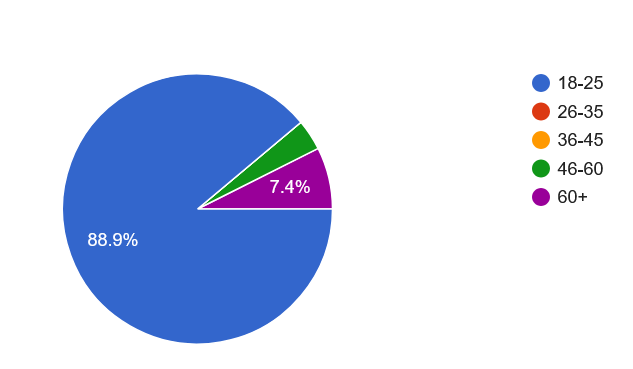
\includegraphics[width=\linewidth]{Screenshot 2026-04-01 232951.png} % replace with actual chart image
\caption{Age group distribution of survey respondents (n=27).}
\label{fig:age}
\end{figure}

\begin{figure}[H]
\centering
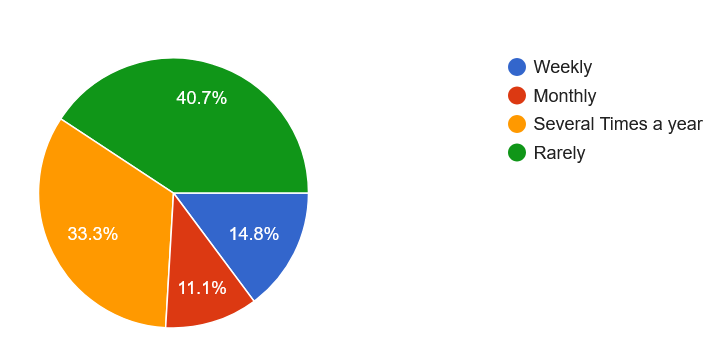
\includegraphics[width=\linewidth]{Screenshot 2026-04-01 233010.png} % replace with actual chart image
\caption{Typical journey duration reported by respondents.}
\label{fig:duration}
\end{figure}

\subsection{Current Train Food Experience}

Figure~\ref{fig:satisfaction} presents passenger satisfaction ratings regarding current train food services. The chart reveals a dismal average rating of 2.07 out of 5, with 44.4\% of users giving the lowest possible score (level 1). Why are we getting such overwhelmingly negative percentages? Open-ended feedback points to a trifecta of systemic failures: unhygienic preparation, stale food, and unjustified high prices. The 44.4\% absolute dissatisfaction rate directly reflects the repetitive nature of these failures—passengers are not experiencing isolated bad meals, but rather a persistent lack of quality control in current railway catering.

Simultaneously, when asked about purchase frequency, 48.1\% report buying train food ``always'' or ``often.'' The reason we observe nearly half the passengers purchasing despite the 44.4\% dissatisfaction rate is a ``captive market'' effect. As noted in the duration chart, passengers are stuck on trains for 6+ hours. They are forced to endure poor-quality food because they have no external alternatives during the journey.

Figure~\ref{fig:waste_obs} shows that an overwhelming 88.9\% of passengers have personally seen food wasted on trains. This specific percentage occurs because current catering models rely on blind bulk-cooking rather than data-driven forecasting. Train pantries overstock perishable items, leading to visible spoilage that passengers observe at the end of the journey.

\begin{figure}[H]
\centering
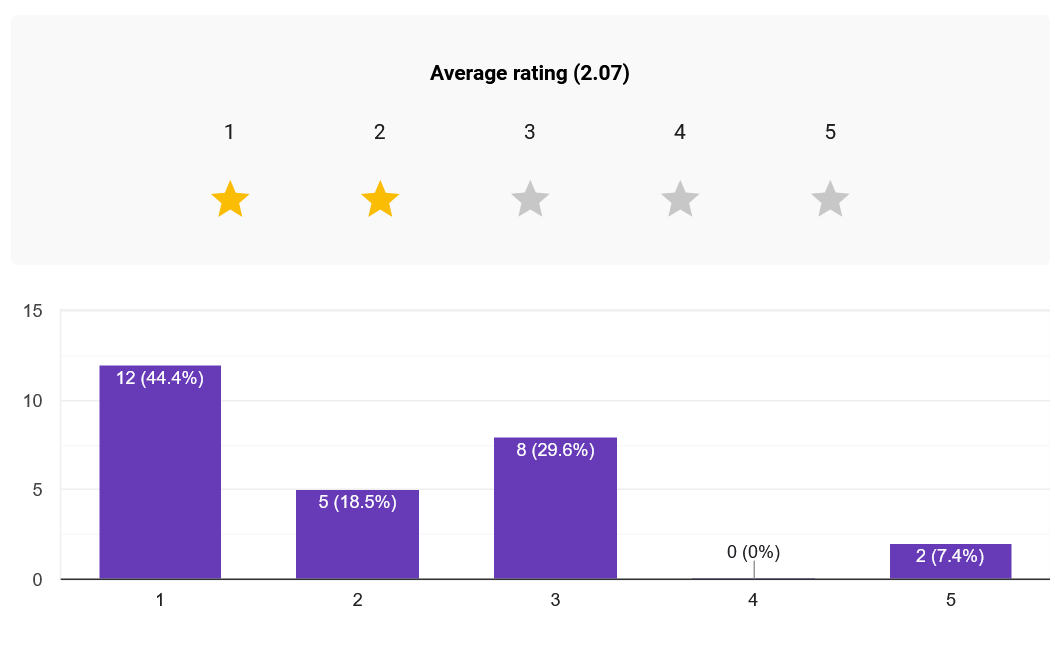
\includegraphics[width=\linewidth]{Screenshot 2026-04-01 233104.png} % replace with actual chart image
\caption{Passenger satisfaction with current train food services (scale 1--5, average = 2.07).}
\label{fig:satisfaction}
\end{figure}

\begin{figure}[H]
\centering
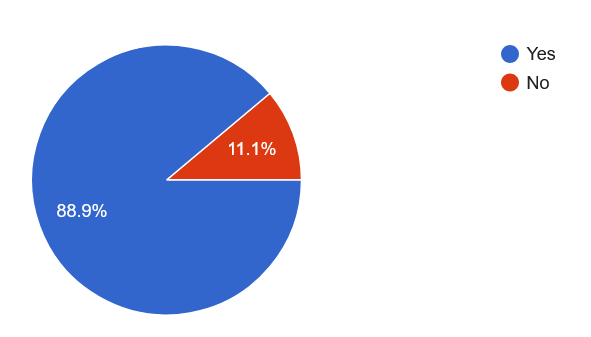
\includegraphics[width=\linewidth]{Screenshot 2026-04-01 233157.png} % replace with actual chart image
\caption{Responses to ``Have you ever seen food wasted on trains?''}
\label{fig:waste_obs}
\end{figure}

\subsection{Mobile Ordering Preferences}

According to Figure~\ref{fig:app}, 51.8\% of users (33.3\% ``Definitely yes'' and 18.5\% ``Probably yes'') intend to use a mobile app for train food. Why are we getting a relatively lukewarm 51.8\% adoption intent, considering the younger demographic? The analysis indicates a significant ``trust deficit.'' Passengers are hesitant to pre-pay for a digital service when the physical food delivery has historically been unreliable. The 33.3\% who are firmly negative or unsure represent a demographic that fears digital failure (e.g., app crashes, failed refunds, or missing orders).

When evaluating feature priorities in Figure~\ref{fig:features}, pre-ordering is the most demanded feature (63\%), closely followed by real-time tracking and reviews (51.9\%). Why are these percentages the highest? Because passengers' primary anxiety is uncertainty. The 63\% demand for pre-ordering exists because passengers want guaranteed food availability before boarding. The 51.9\% demand for tracking occurs because passengers want to know exactly when their food will arrive, eliminating the guesswork associated with current manual trolley services.

\begin{figure}[H]
\centering
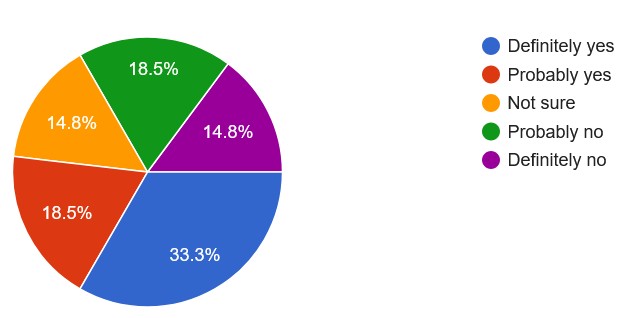
\includegraphics[width=\linewidth]{Screenshot 2026-04-01 233207.png} % replace with actual chart image
\caption{Responses to ``Would you use a mobile app to order food on trains?''}
\label{fig:app}
\end{figure}

\begin{figure}[H]
\centering
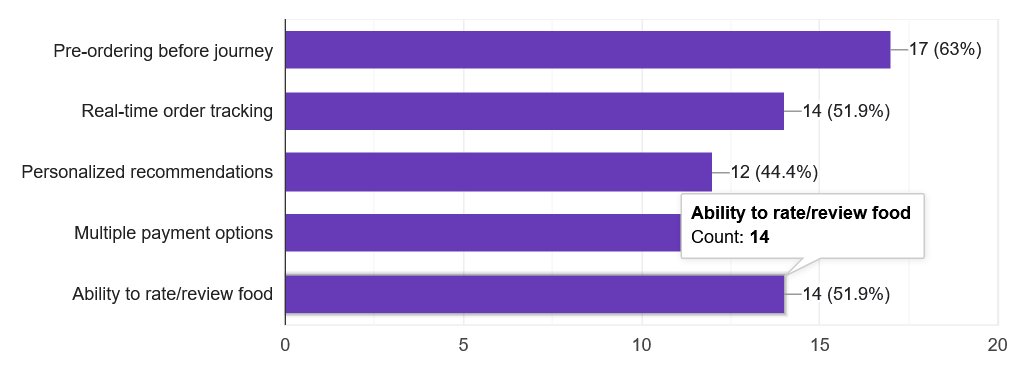
\includegraphics[width=\linewidth]{Screenshot 2026-04-01 233218.png} % replace with actual chart image
\caption{Features that would encourage respondents to use a train food ordering app.}
\label{fig:features}
\end{figure}

\subsection{Food Waste and Sustainability}

Figure~\ref{fig:concern} highlights that 66.6\% of passengers highly rate their concern about food waste (scores of 4 or 5). Why do we see such a strong percentage for environmental awareness? The prevailing visibility of rotting food on trains (as seen in the 88.9\% waste observation rate) naturally elevates passengers' consciousness regarding sustainability. 

However, Figure~\ref{fig:preorder} shows that 59.3\% are unconditionally willing to pre-order to stop waste, while 29.6\% are only conditionally willing. Why do we get this 29.6\% conditional block? The analysis reveals that passengers value convenience over absolute sustainability. They are willing to help the environment, but only if the pre-ordering process does not drastically complicate their ticket booking experience. This highlights the attitude-behavior gap: sustainable intent exists, but the execution must be frictionless.

Furthermore, 59.2\% support dynamic pricing. This percentage exists because younger demographics are accustomed to algorithmic surge/discount pricing from ride-sharing apps, making them receptive to financial incentives that reward early food commitment.

\begin{figure}[H]
\centering
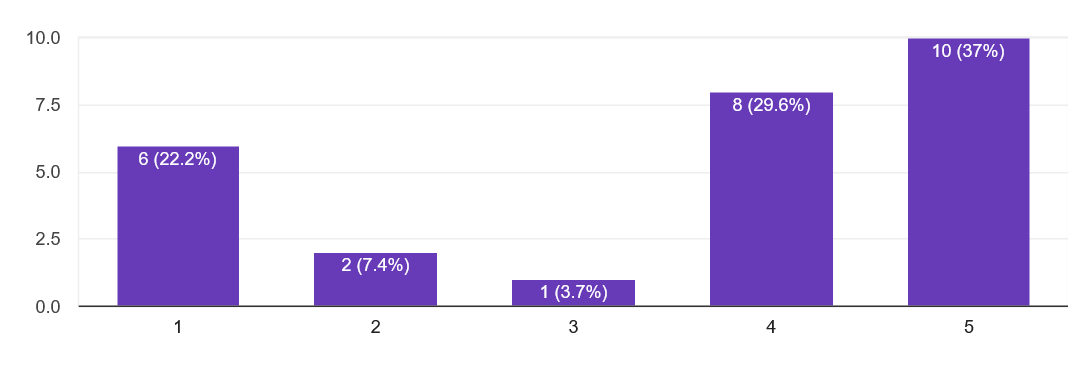
\includegraphics[width=\linewidth]{Screenshot 2026-04-01 233246.png} % replace with actual chart image
\caption{Level of concern about food waste on trains (scale 1--5).}
\label{fig:concern}
\end{figure}

\begin{figure}[H]
\centering
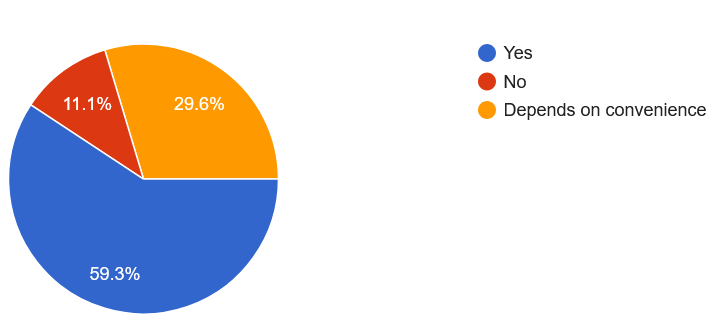
\includegraphics[width=\linewidth]{Screenshot 2026-04-01 233256.png} % replace with actual chart image
\caption{Willingness to pre-order food to help reduce waste.}
\label{fig:preorder}
\end{figure}

\subsection{Transparency and Trust}

Analyzing Figure~\ref{fig:origin}, roughly 77.8\% of passengers explicitly want to know the origin and preparation source of their food. Why are we getting this extremely high percentage? The root cause is a deep-seated fear of foodborne illness. Historically, train food is prepared in unverified external kitchens. The 77.8\% figure represents a protective passenger mechanism—if they know where the food was cooked, they feel safer consuming it.

Figure~\ref{fig:qr} supports this, with 70.3\% showing willingness to scan QR codes for freshness verification. Why do they want QR codes specifically? Digital verification removes human error. Rather than trusting a vendor's verbal claim that the food is fresh, a QR code linked to a digital timestamp provides indisputable proof of the cooking time, effectively overriding the current lack of faith in the catering staff.

Lastly, Figure~\ref{fig:iot} shows that 70.3\% consider real-time IoT temperature tracking highly important (ratings 4 and 5). This percentage directly correlates to the length of the journeys (often 6+ hours). Passengers know that food spoils quickly in transit, and they want IoT tracking to assure them that cold chain or hot storage standards were maintained during the trip.

\begin{figure}[H]
\centering
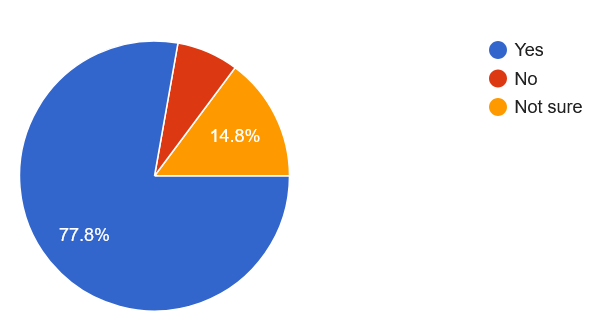
\includegraphics[width=\linewidth]{Screenshot 2026-04-01 233328.png} % replace with actual chart image
\caption{Responses to ``Would you like to see where your food comes from?''}
\label{fig:origin}
\end{figure}

\begin{figure}[H]
\centering
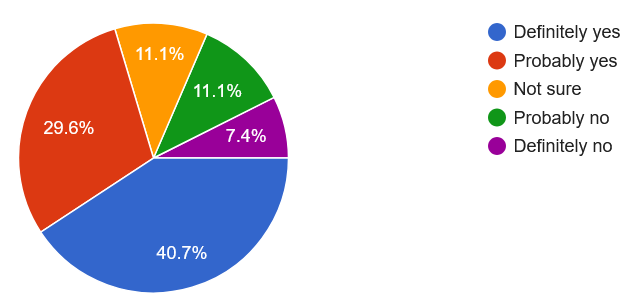
\includegraphics[width=\linewidth]{Screenshot 2026-04-01 233343.png} % replace with actual chart image
\caption{Willingness to use QR code scanning to view food origin and freshness.}
\label{fig:qr}
\end{figure}

\begin{figure}[H]
\centering
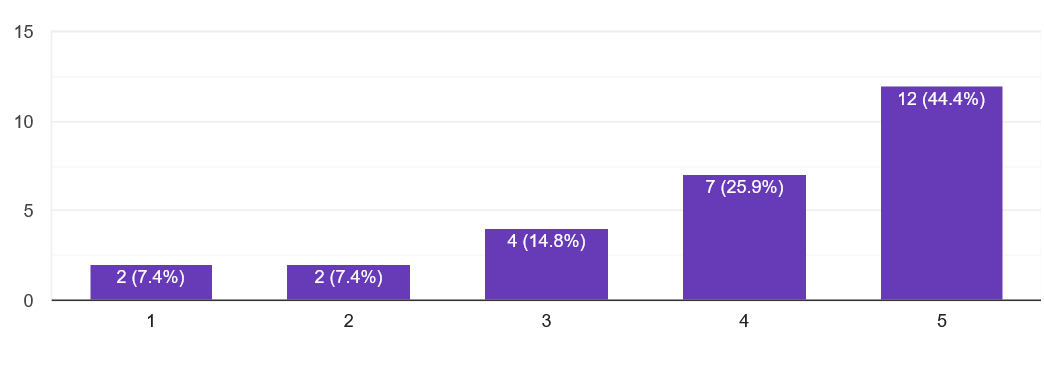
\includegraphics[width=\linewidth]{Screenshot 2026-04-01 233358.png} % replace with actual chart image
\caption{Importance of real-time food quality tracking (e.g., temperature sensors), scale 1--5.}
\label{fig:iot}
\end{figure}

\subsection{Discussion}

The preceding survey analysis across these five themes transitions the focus from merely reporting raw percentages to understanding the underlying behavioral causes. When we compile these causal inferences, several major implications for smart railway food systems emerge, effectively marrying our empirical data with the theoretical literature.

\begin{table}[H]
\centering
\begin{tabular}{|p{3.5cm}|p{1.5cm}|p{2.5cm}|}
\hline
\textbf{Finding} & \textbf{(\%)} & \textbf{Dimension} \\
\hline
Observed food waste on trains & 88.9 & Waste reduction \\
\hline
Pre-order support (yes/conditional) & 88.9 & Demand forecasting \\
\hline
Want food origin info & 77.8 & Traceability \\
\hline
QR code adoption intent & 70.3 & Traceability \\
\hline
IoT quality tracking (rated 4--5) & 70.3 & IoT monitoring \\
\hline
Dynamic pricing support & 59.2 & Cost--waste bridging \\
\hline
Mobile app adoption intent & 51.8 & Consumer satisfaction \\
\hline
\end{tabular}
\caption{Survey findings mapped to research framework dimensions.}
\label{tab:survey-summary}
\end{table}

Why does this integrated picture matter? Because it reveals that a technology-only intervention will fail. The literature review showed that ML-based demand forecasting, smart kitchen waste tracking, and cost--waste analytics can drastically reduce overproduction~\cite{mattila2025,pathway10}. However, our survey reveals an attitude-behavior gap: while sustainability concern is high (66.6\%), mobile app adoption intent is much lower (51.8\%). Passengers will not use a forecasting app unless the physical service regains their trust.

Therefore, the excessive waste observed by 88.9\% of passengers cannot be solved just by deploying an app. The solution requires a bundled approach:
1. \textbf{Demand Forecasting:} Using the 63\% who want pre-ordering as a baseline to predict journey loads, ending the blind-stocking of train pantries.
2. \textbf{Traceability:} Utilizing the 70.3\% demand for QR codes to create a transparent supply chain. If passengers can scan their meal and see that it was cooked two hours ago under hygienic conditions, their baseline dissatisfaction (currently at 44.4\%) will decrease.
3. \textbf{Organizational Overhaul:} Technology must be paired with institutional changes, as noted by the literature~\cite{ijam2025,ce4re2025}. 

By analyzing \textit{why} the charts returned these specific percentages, it is clear that the modern railway passenger is trapped in a constrained-choice environment. A successful smart system must explicitly leverage digital transparency to cure the observed trust deficit, which in turn will drive the pre-ordering behavior needed to permanently eliminate on-board food waste.

%--------------------------------------------------
% 7 Conclusion
%--------------------------------------------------
\section{Conclusion}

This study aimed to conceptualize a smart food ordering and waste reduction framework for railway services by merging theoretical insights from digital food service literature with empirical data from passenger surveys. By thoroughly analyzing the causes behind the survey metrics, we found that immense passenger dissatisfaction and high observable food waste stem directly from a lack of transparency and an outdated, blind-stocking operational model. 

The findings confirm that passengers are highly willing to adopt pre-ordering and QR-based traceability, provided these technical solutions cure their deep-seated distrust regarding food hygiene and availability. Ultimately, addressing these challenges requires shifting from descriptive scenarios to a deeply integrated sociotechnical system. Future research should prioritize pilot implementations of dynamic forecasting and IoT-tracked food pipelines on specific railway routes to validate algorithmic waste reduction alongside improved consumer trust.

\section*{Acknowledgment}
The authors would like to express their sincere gratitude to the faculty members of the Department of Computer Science and Engineering at the Military Institute of Science and Technology for their guidance and constructive feedback throughout this study. The authors are also grateful to the railway passengers who participated in the ``Train Food Service Survey: Passenger Preferences and Feedback'' and generously shared their time and insights, without which the empirical component of this work would not have been possible.

%--------------------------------------------------
% References (IEEE style)
%--------------------------------------------------
\begin{thebibliography}{10}

\bibitem{tarhan2025}
Ç.~Tarhan and B.~Gül, ``Digital traceability in food supply chains: Technologies, benefits, and implementation challenges,'' \emph{J. Food Supply Chain Manag.}, vol.~12, no.~3, pp. 245--267, 2025.

\bibitem{mattila2025}
S.~Mattila, ``Impacts of data-driven demand forecasting in reducing food waste and CO\textsubscript{2} emissions in campus restaurants: A case study,'' \emph{Sustainability in Food Services}, vol.~8, no.~2, pp. 112--134, 2025.

\bibitem{varsini2025}
E.~S. Varsini and K.~M. Ranjani, ``Decoding consumer behavior in online food delivery: A qualitative analysis,'' \emph{J. Digital Consumer Res.}, vol.~15, no.~1, pp. 78--95, 2025.

\bibitem{wjarr2025cold}
``IoT-based real-time monitoring in cold chain food supply,'' \emph{World J. Adv. Res. Rev.}, vol.~19, no.~2, pp. 156--178, 2025.

\bibitem{ijam2025}
``Food waste reduction and digital transformation in institutional food services,'' \emph{Int. J. Appl. Manag.}, vol.~22, no.~4, pp. 301--328, 2025.

\bibitem{benchmark2023}
``Smart kitchen systems and waste monitoring technologies,'' \emph{Food Service Technol. Rep.}, vol.~7, no.~3, pp. 189--215, 2023--2025.

\bibitem{ce4re2025}
``Circular economy and sustainability in food service operations,'' \emph{Eur. Sustain. Initiatives}, vol.~11, no.~2, pp. 234--261, 2024--2025.

\bibitem{wjarr2024blockchain}
``Blockchain applications in agricultural supply chains,'' \emph{World J. Adv. Res. Rev.}, vol.~18, no.~4, pp. 412--438, 2024.

\bibitem{pathway10}
``Mitigating food waste: A new approach to sustainability and cost savings,'' \emph{Business Sustain. Rev.}, vol.~14, no.~1, pp. 67--89, 2025.

\bibitem{envmgmt2025}
``Food waste and environmental management: Holistic assessment approaches,'' \emph{J. Environ. Manag.}, vol.~28, no.~3, pp. 345--372, 2025.

\end{thebibliography}

\end{document}